\chapter{DRI implementation}
\label{cha:implementation}
In the previous chapter, DRI Service architecture was described. In the
following, we present the way how we have implemented it. We also
discuss the technologies that were used for the separate parts of the service.
At the end we briefly descibe how it could be used outside of the VPH-Share
Cloud Platform and integrated in other environment.


\section{Overview}
Implementation of a large software system typically involves some set of
technological or paradigmatic assumptions that have to be taken into
consideration while implementing its components. VPH-Share Cloud Platform takes
advantage of SOA paradigm. All of the components are designed as loosly-coupled web
services that cooperate via REST interfaces. As a~result, each component may
theoretically be implemented using any technology stack. However, to avoid
excessive diversity of software technologies, most of them are implemented in
Java or Ruby programming languages, the practically proven open source
solutions.\\

As it was mentioned in section \ref{cloud-platform}, all of the Cloud
Platform's core services will be deployed within Atomic Service instances,
a VPH-Share application container. Atomic Service can be simply viewed as VM
with add-on software and mechanism installed, such as security or federated
data access layers.\\

DRI Service implementation was conducted according to the architecture
described in chapter \ref{cha:architecture} with the best software development
practices, such as testing and design patterns in mind. The main goal is to
achieve the highest possible data validation efficiency, while providing an
acceptable probability of unavailability or error detection. The design of DRI
Service already solved some performance issues, mostly on the validation
algorithm. However, implementation details have to be taken into account.
	
\section{Implementation challenges and decisions}

It is a recurring engineering truth, that practical implementation to some degree
always affects the design. Ideally, project's implementation should accurately reflect
its design. However, different technology stack choices vary significantly, from
programming language paradigm and available contructs, to best practices and design
patterns, to available libraries and their specifics. Therefore, DRI architecture
presented in chapter \ref{cha:architecture} represents only the the conceptual and
functional view of the service.\\

With DRI Service architecture design we clearly identified the biggest software
engineering challenges that have to be addressed in the implementation. There
are the following:

\begin{itemize}
\item creating REST web service interface (REST producer),
\item REST interoperability with other components (REST consumer),
\item federated cloud access to various cloud storage providers (often non-compatible interfaces),
\item periodic job execution and scheduling,
\item loose coupling between the subcomponents (facilitates configurability and reuse).
\end{itemize}

We have also foreseen, that Cloud Platform components will be changing rapidly
their interfaces and remaining up-to-date will require a lot of integration testing.
It was addressed partially in the DRI architecture, where all of the external service
interactions are wrapped into easily interchangable interfaces (MetadataAccess for example).
Moving with the times, DRI Service implementation was made according to
test driven development (TDD \cite{tdd, tdd-java}) approach to software engineering. 
Broad set of integration sets created this way allowed to spot changes in
other components.

\section{Implementation technologies}
Java programming language \cite{java-language} was chosen as implementation
language and technology stack. Advantages are significant, Java:

\begin{itemize}
\item proved to be high-performance and commercially proven,
\item has a vast number of libraries available,
\item has big and active community,
\item has wealth range of developer tools.
\end{itemize}

At its core, DRI Service is a Java Servlet \cite{java-servlet}
component which accepts REST requests on specified URI paths and performs the
requested task utilizing MetadataAccess, ValidationExecutor, 
ReplicationExecutor, ValidationStrategy and FederatedDataAccess, implemented as
simple Java objects. In Java Servlet model, the programmer is free of the
object's lifecycle management and REST/HTTP communication complexities, which
is provided by the container into which application is deployed.\\

Another important implementation's aspect is dependency injection (DI \cite{di,di-book}). It is
a~software design pattern which releases the programmer from "dependency-hell"
problem. It removes the need to provide dependencies (object instances) when
constructing objects, which is error-prone. Dependencies are provided
dynamically by the DI container at runtime according to the configuration.
In DRI, we use Guice library \cite{guice} for DI capabilities. DI approach
significantly simplifies component's testing in a service-based environment as
dependable service can be simply swapped with a~mock object in the
configuration.\\

DRI Service components implementation technologies are depicted in figure
\ref{fig:dri-impl-technologies}. Further subsections describe them in detail.

\begin{figure}[h!]
	\centering
	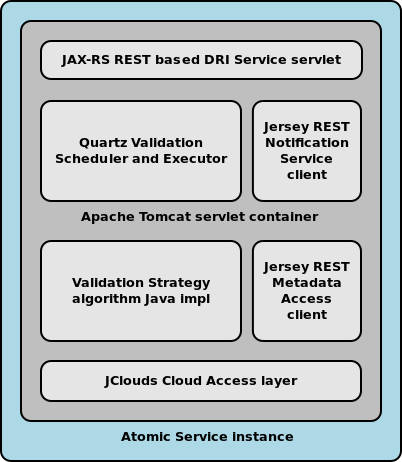
\includegraphics[width=0.5\textwidth]{images/dri-impl-technologies.png}
	\caption{DRI Service implementation technologies of its modules. REST API
	interface is provided using JAX-RS technology. Federated data access is built
	on JClouds library which abstracts the complexity of accessing different cloud
	storage providers. Jersey REST client library eases the integration with REST
	based services on which DRI depends. Finally, in batch execution DRI utilizes
	Quartz library.}
	\label{fig:dri-impl-technologies}
\end{figure}
 
\subsection{REST interfaces}
To provide REST interface and cooperate with other Cloud Platform
components, DRI utilizes Jersey library \cite{jersey} -- a reference
implementation of the JAX-RS specification \cite{jax-rs} and supports seamless
integration with Java Servlet technology. It provides both, server and client
REST interoperability via Java annotations \cite{jls}.\\

\subsubsection{Server side}
In JAX-RS to create a REST interface for DRI it is as simple as the following:
Creating JAX-RS based REST service interfaces is very simple. The following
listing shows a part of the DRIService interface:

\lstinputlisting[language=Java, basicstyle=\footnotesize, frame=single]{src/DRIService.java}

To make your Java method available through REST you simply annotate the class and its methods with
JAX-RS annotations. Let us take \textit{getManagedDataset} method as an example. It will

\begin{enumerate}
\item be available under \textit{/driservice/get\_managed\_dataset/{datasetId}} URL,
where \textit{datasetId} is a string part of the URL specifying dataset id (\textit{Path} annotation),
\item be accessible via HTTP GET method (\textit{GET} annotation),
\item produce HTTP JSON format output (\textit{Produces} annotation).
\end{enumerate}

The format of the \textit{ManagedDataset} JSON method output is mapped into Java object
via \textit{XmlRootElement} and \textit{XmlElement} JAXB annotations \cite{jaxb}.
 
\subsubsection{Client side}
Creating Jersey based client of the REST service is also straight-forward:

\lstinputlisting[language=Java, basicstyle=\footnotesize, frame=single]{src/AIRMetadataRegistry.java}

Here, we use already configured \textit{WebResource} object to build REST query to 
\textit{BASE\_URL/get\_datasets} URL with \textit{only\_managed} query parameter. Jersey
automatically deserialize the returned response into \textit{ManagedDataset} object
we presented in the previous listing.\\

\subsection{Cloud storage access}
Current cloud storage services mostly provide a~standard REST interface.
Despite interface similarities, it appears cumbersome to support the
differences between providers. To get rid of this problem, DRI uses JClouds
\cite{jclouds} library that provides a~common API layer that abstracts cloud
dissimilarities. Thus, access to the cloud storage federation is quite easy
via programmer perspective. At the time of writing this thesis, JClouds
supports up to 30 different cloud providers including Amazon, GoGrid, vCloud,
Openstack, Azure and others. Storage access is provided as Blobstore API, which
incorporates three concepts: service, container and blob. The Blobstore is
a~key-value store such as Amazon S3, where your account exists and where you
can create containers. A container is a namespace for you data and many of them
can exist. Blob is an unstructued data stored in a container referenced by
its name. In all cloud storages, the combination of the account, container and
blob relates directly to the HTTP URL. Access to data can be performed
synchronously or asynchronously, depending on the selected Blobstore type.
While Blobstore API provides cloud storage abstraction it cannot overcome
specific cloud provider's limitations, for example size limits or timeouts
between sensitive operations.\\

JClouds's Blobstore abstraction provides uniform interface to different cloud storage
providers. To use provider \textit{X} one have to create \textit{BlobStoreContext}
for \textit{X}. The following snippet simply shows how to access Amazon S3, create a
container and put a blob into it:

\lstinputlisting[language=Java, basicstyle=\footnotesize, frame=single]{src/jclouds-example.java}

\subsection{Request and periodic task scheduling}
DRI Service periodically monitors data integrity. Periodic tasks invocation
is a~recurring issue in many IT systems. DRI uses Quartz library \cite{quartz}
for task scheduling and execution. Quartz is a~full-featured open source job scheduling
library that can be integrated with, or used along side virtually any Java
application -- from the smallest to the largest e-commerce system. Its main highlights
are the following:

\begin{itemize}
\item periodic and timer jobs,
\item configurable executors (single thread or pool of threads),
\item templates for creating job task objects,
\item support for job transactions and persistence, 
\item scalable -- from simple to complex schedules for executing tens, hundreds 
or even ten-of-thousands of jobs,
\end{itemize}

DRI Service uses Quartz in the following way: at startup it schedules main (root)
periodic job with specified period, which upon trigger, is responsible for scheduling
one validation job per managed dataset. Apart from periodic validation, the dataset's 
integrity check can be performed on request. In such case, DRI tries to add validation
job for the specified dataset to the schedule. If a~job with the same dataset id
already exists in the queue, nothing happens (double validation is not desired). Otherwise, 
the job with specified dataset id is added to the schedule. Worth mentioning is the fact,
that apart from validation jobs, there are jobs that update dataset checksums whenever its
contents changed and both of them cannot collide with each other. Upon job execution, a
\textit{JobDetail} is returned.

\section{Validation implementation details}
DRI Service utilizes efficient data validation algorithm to achieve acceptable
performance over large amount of data. However, apart from algorithm
efficiency, its optimized implementation is greatly desirable. Due to the fact
that the validation algorithm is highly oriented on network communication (see
section \ref{section:validation-algorithm}), network bandwidth and latency are
the most significant factors affecting its performance. The point of the
biggest interest is access to large number of the selected chunks of data. As
it was noted in section \ref{cloud-model}, current cloud storage interfaces do
not enable efficient way to perform this operation. However, even though
individual chunks of data have to be requested in separate HTTP calls, they can
be invoked asynchronously in parallel to reduce round-trip time (RTT) latency.
DRI employs this scheme via asynchronous Blobstore API provided by JClouds
library. When DRI validates single logical data within dataset, it invokes
a~configurable number of asychronous data chunks requests and then waits for
their completion. The scheme repeats until all the needed chunks for logical
data are collected.\\

\section{Deployment environment}
Currently, at proof of concept stage, the DRI is deployed on Apache Tomcat
\cite{apache-tomcat} instance which runs on virtual machine (VM). However, in
full-operational Cloud Platform it will be deployed within Atomic Service
instance (simply a VM with some add-ons) as one of its core services. Apache
Tomcat is a web application container which implements Java Servlet
specification and provides its application environment. Nevertheless, any other
application server compliant with Java Servlet specification can be used.

\section{The use outside of Cloud Platform}
DRI Service component could be successfully used outside of the VPH-Share Cloud Platform
frame. By design, its dependent components are used through abstraction layers and could
be easily swapped to accomodate to other environment. Metadata could be stored on
cloud storage or local disk file; Notification Service could be implemented as a mail sender
or chat client -- every such change requires only to modify one package (see figure 
\ref{fig:dri-ability-to-change}. Moreover, many of the configuration parameters such as:
REST urls, credentials, federated cloud metadata etc, are kept in configuration file and
can be easily changed.

\begin{figure}[h!]
	\centering
	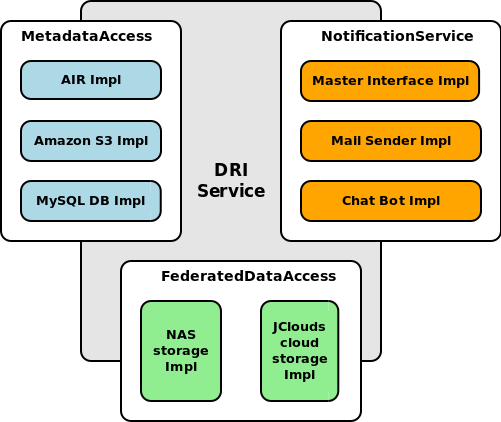
\includegraphics[width=0.6\textwidth]{images/DRI-ability-to-change.png}
	\caption{Possibility to switch DRI service providers by reimplementing abstraction
	layer and accomodate to new environment, other than VPH-Share Cloud Platform}
	\label{fig:dri-ability-to-change}
\end{figure}

\section{Scalability} 
It is foreseen, that with the growth of the platform it could be necesarry for DRI to
provide scalable solution. Hopefully, by design, DRI is a stateless web service so the
simplest solution would be to run a couple of its instances and provide requests load
balancing between them. Another possibility, as DRI uses Quartz for job scheduling and
execution, would be to build Quartz cluster and make DRI submit its validation jobs
to it. Lastly, single dataset (or even single file) validation is completely independent
from one another, meaning that scalability issues can be easily addressed.

\section{Summary}
This chapter presented the way DRI service was implemented based on its design and
requirements described in the previous chapter. It outlines the choice of Java technology stack
and additional libraries and justifies it. JClouds library helped us to address one of the
main implementation challenges to abstract cloud storage access and get rid of cloud provider
interface differences. Additionally, JAX-RS, Guice and Quartz enabled us to create the skeleton
of DRI implementation relatively fast and without complications. At the end we also discuss
the possiblitity to use DRI outside of VPH-Share platform. To achieve this, one has to reimplement
the abstract layer through which DRI accesses external services. On the other hand, scalability can
be easily achieved by small modifications through running multiple instances of DRI service and
pinning datasets periodical validations to concrete instances.
